%\documentclass[12pt]{article}

\questionheader{ex:s1.1}


%%%%%%%%%%%%%%%%%%
\subsection*{\Conceptual}
%%%%%%%%%%%%%%%%%%

%%%%%%%%%%%%%%%%%%%%%%%%%%%%
%\Instructions{Questions~\ref{prob_s1.0first} through \ref{prob_s1.0last} provide practice with.}
%%%%%%%%%%%%%%%%%%%%

%%%%%%%%%%%%%%%%%%%%%%%%%%%%%%%%
\begin{question}
 Describe the set of all points $(x,y,z)$ 
in $\bbbr^3$ that satisfy
\begin{enumerate}[(a)] 
\item
          $x^2 +y^2+z^2= 2x-4y+4$
\item
          $x^2 +y^2+z^2< 2x-4y+4$
\end{enumerate}
\end{question}

%\begin{hint}
%
%\end{hint}

\begin{answer}
(a) The sphere of radius 3 centered on $(1,-2,0)$.

(b) The interior of the sphere of radius 3 centered on $(1,-2,0)$.

\end{answer}

\begin{solution}
(a) The point $(x,y,z)$ satisfies $x^2 +y^2+z^2= 2x-4y+4$
if and only if it satisfies $x^2-2x +y^2+4y+z^2= 4$, or equivalently 
$(x-1)^2 +(y+2)^2+z^2=9 $. Since $\sqrt{(x-1)^2 +(y+2)^2+z^2}$ is the distance
from $(1, -2, 0)$ to $(x,y,z)$, our point satisfies the given equation
if and only if its distance from $(1,-2,0)$ is three. So the set is
the sphere of radius 3 centered on $(1,-2,0)$.

(b)
As in part (a), $x^2 +y^2+z^2< 2x-4y+4$
if and only if  $(x-1)^2 +(y+2)^2+z^2<9 $. Hence our point 
satifies the given inequality
if and only if its distance from $(1,-2,0)$ is strictly smaller than three. 
The set is the interior of the sphere of radius 3 centered on $(1,-2,0)$.

\end{solution}

%%%%%%%%%%%%%%%%%%%%%%%%%%%%%%%%%%%%
\begin{question}
Describe and sketch the set of all points $(x,y)$ 
in $\bbbr^2$ that satisfy
\begin{enumerate}[(a)]
\item
$x=y$
\item
$x+y=1$
\item
$x^2+y^2=4$
\item
$x^2+y^2=2y$
\item
$x^2+y^2<2y$
\end{enumerate}
\end{question}

\begin{hint}
In part (d), complete a square.
\end{hint}

\begin{answer}
(a) $x=y$ is the straight line through the origin that makes an 
angle $45^\circ$ with the $x$-- and $y$--axes. It is sketched in the 
figure on the left below.

\begin{center}
     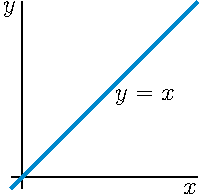
\includegraphics{sec1_1_Q1a.pdf}\qquad\qquad
     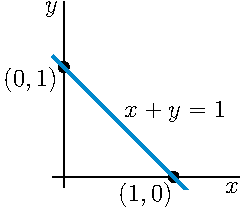
\includegraphics{sec1_1_Q1b.pdf}
\end{center}

(b) $x+y=1$ is the straight line through the points $(1,0)$ and
$(0,1)$. It is sketched in the figure on the right above.

(c) $x^2+y^2=4$ is the circle with centre $(0,0)$ and radius 2. It is 
sketched in the figure on the left below.

\begin{center}
     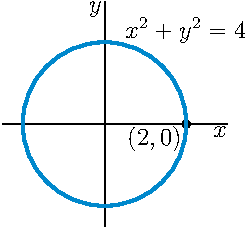
\includegraphics{sec1_1_Q1c.pdf}\qquad\qquad
     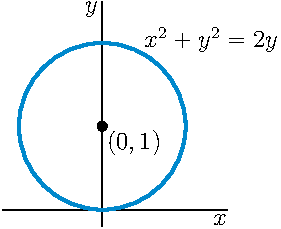
\includegraphics{sec1_1_Q1d.pdf}
\end{center}

(d) $x^2+y^2=2y$ is the circle with centre $(0,1)$ and radius 1.
It is sketched in the figure on the right above.

(e) $x^2+y^2<2y$ is the set of points that are strictly inside 
the circle with centre $(0,1)$ and radius 1.
It is the shaded region (not including the dashed circle) in the sketch below.

\begin{center}
     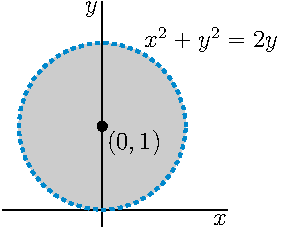
\includegraphics{sec1_1_Q1e.pdf}
\end{center}

\end{answer}

\begin{solution}
(a) $x=y$ is a straight line and passes through the points $(0,0)$
and $(1,1)$. So it is the straight line through the origin that makes an angle $45^\circ$ with the $x$-- and $y$--axes. It is sketched in the figure on the 
left below.

\begin{center}
     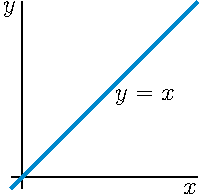
\includegraphics{sec1_1_Q1a.pdf}\qquad\qquad
     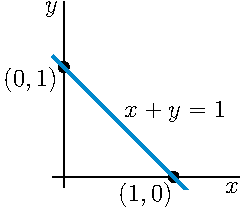
\includegraphics{sec1_1_Q1b.pdf}
\end{center}

(b) $x+y=1$ is the straight line through the points $(1,0)$ and
$(0,1)$. It is sketched in the figure on the right above.

(c) $x^2+y^2$ is the square of the distance from $(0,0)$ to $(x,y)$.
So $x^2+y^2=4$ is the circle with centre $(0,0)$ and radius 2.
It is sketched in the figure on the left below.

\begin{center}
     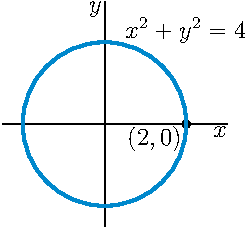
\includegraphics{sec1_1_Q1c.pdf}\qquad\qquad
     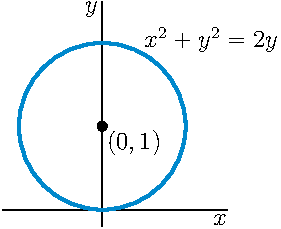
\includegraphics{sec1_1_Q1d.pdf}
\end{center}

(d) The equation $x^2+y^2=2y$ is equivalent to  $x^2+(y-1)^2=1$.
As $x^2+(y-1)^2$ is the square of the distance from $(0,1)$ to $(x,y)$,
$x^2+(y-1)^2=1$ is the circle with centre $(0,1)$ and radius 1.
It is sketched in the figure on the right above.

(e) As in part (d),
\begin{equation*}
x^2+y^2<2y
\iff x^2+y^2-2y<0
\iff x^2+y^2-2y+1<1
\iff x^2+(y-1)^2<1
\end{equation*}
As $x^2+(y-1)^2$ is the square of the distance from $(0,1)$ to $(x,y)$,
$x^2+(y-1)^2<1$ is the set of points whose distance from $(0,1)$ is 
strictly less than $1$. That is, it is the set of points strictly inside 
the circle with centre $(0,1)$ and radius 1.
That set is the shaded region (not including the dashed circle) 
in the sketch below.

\begin{center}
     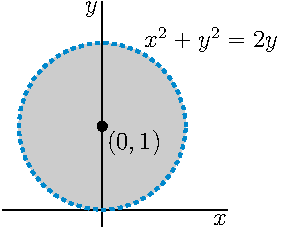
\includegraphics{sec1_1_Q1e.pdf}
\end{center}
\end{solution}

%%%%%%%%%%%%%%%%%%%%%%%%%%%%%%%%%%%%%%
\begin{question}
Describe the set of all points $(x,y,z)$ in $\bbbr^3$ that satisfy
the following conditions. Sketch the part of the set that is in the 
first octant.
\begin{enumerate}[(a)]
\item
$z = x$
\item
$x + y + z = 1$
\item
$x^2 + y^2 + z^2 = 4$
\item
$x^2 + y^2 + z^2 = 4$, $z = 1$
\item
$x^2+y^2=4$
\item
$z = x^2 + y^2$
\end{enumerate}
\end{question}

%\begin{hint}
%
%\end{hint}


\begin{answer}
(a)
The set $z=x$ is the plane which contains the $y$--axis and which  
makes an angle $45^\circ$ with the $xy$--plane. Here is a sketch 
of the part of the plane that is in the first octant.

\begin{center}
     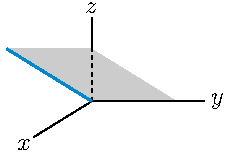
\includegraphics{xeqzPlane.pdf}
\end{center}


(b)
$x+y+z=1$ is the plane through the points $(1,0,0)$, $(0,1,0)$
and  $(0,0,1)$. Here is a sketch of the part of the plane 
that is in the first octant.

\begin{center}
     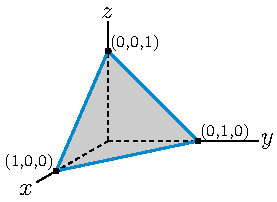
\includegraphics{xyzPlane.pdf}
\end{center}


(c)
$x^2+y^2+z^2=4$ is the sphere with centre $(0,0,0)$ and radius 2.
Here is a sketch of the part of the sphere that is in the first octant.

\begin{center}
     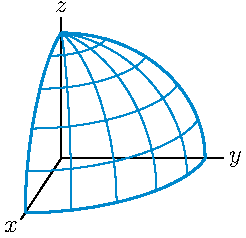
\includegraphics{quarterSphere.pdf}
\end{center}

(d)
$x^2+y^2+z^2=4$, $z=1$ is the circle in the plane $z=1$ 
that has centre $(0,0,1)$ and radius $\sqrt{3}$. The part of the circle
in the first octant is the heavy quarter circle in the sketch

\begin{center}
     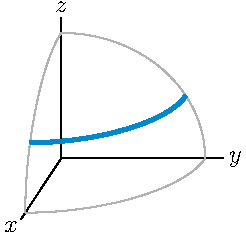
\includegraphics{quarterCircle.pdf}
\end{center}


(e)
$x^2+y^2=4$ is the cylinder of radius $2$ centered on the $z$--axis.
Here is a sketch of the part of the cylinder that is in the first octant.

\begin{center}
     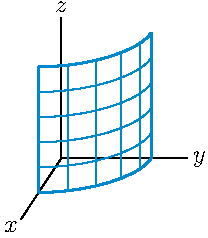
\includegraphics{quarterCylinder.pdf}
\end{center}


(f) $z=x^2+y^2$ is a paraboloid consisting of a vertical stack of 
horizontal circles. The intersection of the surface with the $yz$--plane 
is the parabola $z=y^2$.  Here is a sketch of the part of the paraboloid 
that is in the first octant.

\begin{center}
     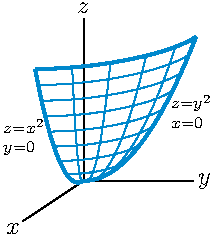
\includegraphics{quarterParaboloid.pdf}
\end{center}

\end{answer}


\begin{solution}
(a) 
For each fixed $y_0$, $z=x,\ y=y_0$ is a straight line 
that lies in the plane, $y=y_0$ (which is parallel to the plane 
containing the $x$ and $z$ axes and is a distance $y_0$ from it). 
This line passes through $x=z=0$ and makes an angle $45^\circ$ 
with the $xy$--plane. Such a line (with $y_0=0$) is sketched in the 
figure below.
The set $z=x$ is the union of all the lines $z=x,\ y=y_0$ with all 
values of $y_0$. As $y_0$ varies  $z=x,\ y=y_0$ sweeps out the 
plane which contains the $y$--axis and which  makes an angle 
$45^\circ$ with the $xy$--plane. Here is a sketch of the part of the plane 
that is in the first octant.

\begin{center}
     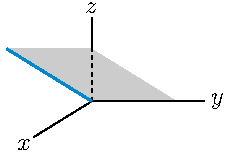
\includegraphics{xeqzPlane.pdf}
\end{center}


(b) 
$x+y+z=1$ is the plane through the points $(1,0,0)$, $(0,1,0)$
and  $(0,0,1)$. Here is a sketch of the part of the plane 
that is in the first octant.

\begin{center}
     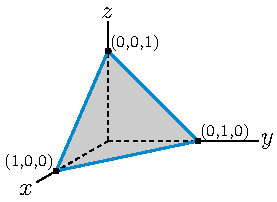
\includegraphics{xyzPlane.pdf}
\end{center}

(c)
  $x^2+y^2+z^2$ is the square of the distance from $(0,0,0)$ to $(x,y,z)$.
So $x^2+y^2+z^2=4$ is the set of points whose distance from $(0,0,0)$ is
$2$. It is the sphere with centre $(0,0,0)$ and radius 2.
Here is a sketch of the part of the sphere that is in the first octant.

\begin{center}
     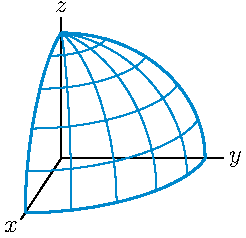
\includegraphics{quarterSphere.pdf}
\end{center}

(d) 
$x^2+y^2+z^2=4$, $z=1$ or equivalently $x^2+y^2=3$, $z=1$,
is the intersection of the plane $z=1$ with the sphere of centre 
$(0,0,0)$ and radius 2. It is a circle in the plane $z=1$ 
that has centre $(0,0,1)$ and radius $\sqrt{3}$. The part of the circle
in the first octant is the heavy quarter circle in the sketch

\begin{center}
     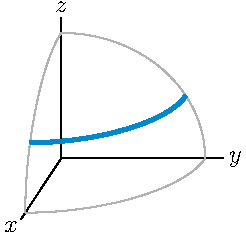
\includegraphics{quarterCircle.pdf}
\end{center}

(e) 
For each fixed $z_0$, $x^2+y^2=4$, $z=z_0$ is a circle in the 
plane $z=z_0$ with centre $(0,0,z_0)$ and radius $2$. 
So $x^2+y^2=4$ is the union of $x^2+y^2=4,\ z=z_0$ for all 
possible values of $z_0$. It is  a vertical stack of horizontal 
circles. It is the cylinder of radius $2$ centered on the $z$--axis.
Here is a sketch of the part of the cylinder that is in the first octant.

\begin{center}
     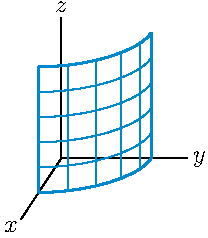
\includegraphics{quarterCylinder.pdf}
\end{center}


(f)
For each fixed $z_0\ge 0$, the curve $z = x^2 + y^2,\ z=z_0$ is the circle in the plane $z=z_0$ with centre $(0,0,z_0)$ and radius $\sqrt{z_0}$. As 
$z = x^2 + y^2$ is the union of $z = x^2 + y^2,\ z=z_0$ for all 
possible values of $z_0\ge 0$, it is  a vertical stack of horizontal circles.
The intersection of the surface with the $yz$--plane is the parabola
$z=y^2$.  Here is a sketch of the part of the paraboloid that is in the 
first octant.

\begin{center}
     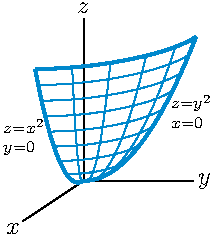
\includegraphics{quarterParaboloid.pdf}
\end{center}


\end{solution}




%%%%%%%%%%%%%%%%%%
\subsection*{\Procedural}
%%%%%%%%%%%%%%%%%%


\begin{question}
Consider any triangle. Pick a coordinate system so that one vertex
is at the origin and a second vertex is on the positive $x$--axis. Call
the coordinates of the second vertex $(a,0)$ and those of the third vertex
$(b,c)$. Find the circumscribing circle (the circle that goes through all
three vertices).
\end{question}

%\begin{hint}
%
%\end{hint}


\begin{answer}
The circumscribing circle has centre $(\bar x,\bar y)$ and radius $r$
with $\bar x=\frac{a}{2}$, $\bar y=\frac{b^2+c^2-ab}{2c}$ and
$r=\sqrt{\big(\frac{a}{2}\big)^2+\big(\frac{b^2+c^2-ab}{2c}\big)^2}$.
\end{answer}


\begin{solution}
Call the centre of the circumscribing circle 
$(\bar x,\bar y)$. This centre must be equidistant from the three vertices.
So
\begin{equation*}
\bar x^2+\bar y^2=(\bar x-a)^2+\bar y^2=(\bar x-b)^2+(\bar y-c)^2 
\end{equation*}
or, subtracting $\bar x^2+\bar y^2$ from the three equal expressions,
\begin{equation*}
0=a^2-2a\bar x=b^2-2b\bar x+c^2-2c\bar y
\end{equation*}
which implies
\begin{equation*}
\bar x=\frac{a}{2}\qquad\qquad \bar y
=\frac{b^2+c^2-2b\bar x}{2c}=\frac{b^2+c^2-ab}{2c}
\end{equation*}
The radius is the distance from the vertex $(0,0)$ to the centre 
$(\bar x,\bar y)$, which is
$\sqrt{\big(\frac{a}{2}\big)^2+\big(\frac{b^2+c^2-ab}{2c}\big)^2}$.

\end{solution}

%%%%%%%%%%%%%%%%%%%%%%%%%%%%%%%%%%%%%%%%%
\begin{question} [M200 2001A] % 1
A certain surface consists of all points $P=(x,y,z)$
such that the distance from $P$ to the point $(0,0,1)$ is equal to the
distance from $P$ to the plane $z+1=0$. Find an equation for the surface,
sketch and describe it verbally.
\end{question}

%\begin{hint}
%
%\end{hint}

\begin{answer}
$x^2+y^2=4z$
The surface is a paraboloid consisting of a stack of horizontal circles, starting with a point at the origin and with radius increasing vertically.
The circle in the plane $z=z_0$ has radius $2\sqrt{z_0}$.
\end{answer}

\begin{solution}
The distance from $P$ to the point $(0,0,1)$ is $\sqrt{x^2+y^2+(z-1)^2}$.
The distance from $P$ to the specified plane is $|z+1|$. Hence the equation
of the surface is
\begin{equation*}
x^2+y^2+(z-1)^2=(z+1)^2\text{ or }
   x^2+y^2=4z
\end{equation*}
All points on this surface have $z\ge 0$. The set of points on the surface
that have any fixed value, $z_0\ge 0$, of $z$ consists of a circle that is
centred on the $z$--axis, is parallel to the $xy$-plane and has radius
$2\sqrt{z_0}$. The surface consists of a stack of these circles, starting
with a point at the origin and with radius increasing vertically. The surface
is a paraboloid and is sketched below.
\begin{center}
     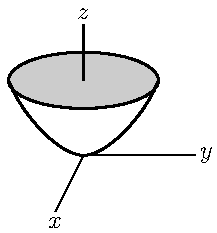
\includegraphics{OE01AQ1.pdf}
\end{center}
\end{solution}



%%%%%%%%%%%%%%%%%%
\subsection*{\Application}
%%%%%%%%%%%%%%%%%%

\begin{question}
The pressure $p(x,y)$ at the point $(x,y)$ is at least zero and is 
determined by the equation $x^2-2px+y^2=3p^2$. Sketch several isobars. 
An isobar is a curve with equation $p(x,y)=c$ for some constant $c\ge 0$.
\end{question}

\begin{hint}
It is not necessary to solve the equation $x^2-2px+y^2=3p^2$ for $p(x,y)$.
For example, a point $(x,y)$ is on the isobar $p(x,y)=1$ if and only if
$x^2-2x+y^2=3$. This curve can be easily identified if one first completes a 
square.
\end{hint}


\begin{answer}
\begin{center}
     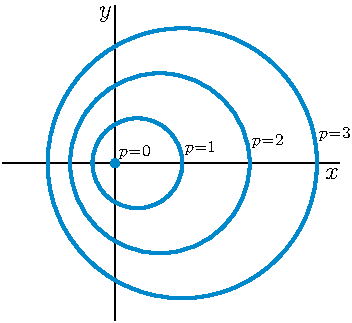
\includegraphics{pressureB.pdf}
\end{center}

\end{answer}


\begin{solution}
For each fixed $c\ge 0$, the isobar $p(x,y)=c$ is the curve
$x^2-2cx+y^2=3c^2$, or equivalently, $(x-c)^2+y^2=4c^2$. This is a 
circle with centre $(c,0)$ and radius $2c$. Here is a sketch of the isobars
$p(x,y)=c$ with $c=0,1,2,3$.

\begin{center}
     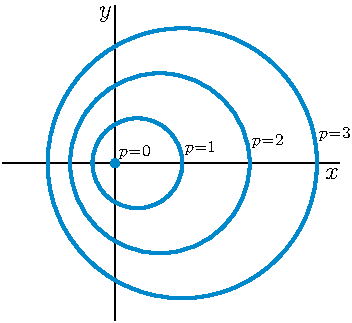
\includegraphics{pressureB.pdf}
\end{center}


\end{solution}
